\section{Modeling: Theory and Simulation}\label{cha:plasma modeling}
    When modeling fluids, there exist 3 classes of models (in so far as will be considered in this thesis):
    \begin{enumerate}
        \item  Particle models (See Definition \ref{def:particle model})
        \item  Kinetic models (See Definition \ref{def:kinetic model})
        \item  Fluid models (See Definition \ref{def:fluid model})
    \end{enumerate}
    When constructing a model, one starts from the full particle model, making assumptions on that model to reduce it to a kinetic model, and making further assumptions to reduce it to a fluid model. When progressing along this route, while the models become simpler in dimension, easing their analysis and numerical simulation, further and greater assumptions are required. One therefore finds a trade-off between the simplicity and approachability of the model, and its efficacy for the fluid being modeled.
    
    \begin{center}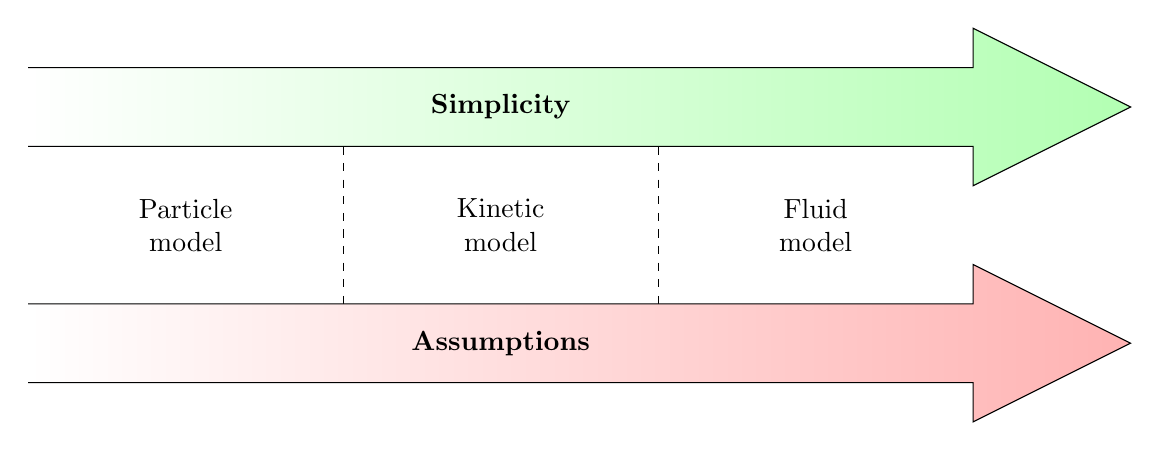
\begin{tikzpicture}[align = center, node distance = 4cm, auto]
        \node at (0, 0) {Particle \\ model};
        \node at (4, 0) {Kinetic  \\ model};
        \node at (8, 0) {Fluid    \\ model};

        \draw[dashed] (2, 1) -- (2, - 1);
        \draw[dashed] (6, 1) -- (6, - 1);
        
        \draw[left color = white, right color = green!30!white]
            (- 2, 1) -- (10, 1) -- (10, 0.5) -- (12, 1.5) -- (10, 2.5) -- (10, 2) -- (- 2, 2);
        \node at (4, 1.5) {\bf Simplicity};
        
        \draw[left color = white, right color = red!30!white]
            (- 2, - 1) -- (10, - 1) -- (10, - 0.5) -- (12, - 1.5) -- (10, - 2.5) -- (10, - 2) -- (- 2, - 2);
        \node at (4, - 1.5) {\bf Assumptions};
    \end{tikzpicture}\end{center}

    For classical single phase, electrically-neutral fluids under typical real-world conditions, these assumptions are almost wholly valid, leading to the Navier--Stokes (NS) equations. When the same steps are applied for a quasineutral plasma, one derives the magnetohydrodynamic (MHD) equations.
    
    Under typical tokamak-like conditions however, the steps required to go from the kinetic model to the fluid model do not hold nearly as well. Full fluid models like the MHD equations fail to capture highly influential ``kinetic effects'', which are necessarily present only in the full kinetic model, which are highly influential in tokamak plasma dynamics. These include:
    \begin{itemize}
        \item  Most plasma waves \BA{[Ref]}
        \item  Most plasma/kinetic instabilities \BA{[Ref]}
        \item  Landau damping/Bump-on-tail instabilities \BA{[Ref]}
        \item  Leakage \BA{[Ref]}
        \item  Kinetic structures (Beams/Double layers) \BA{[Ref]}
        \item  Anisotropic pressures \BA{[Ref]}
    \end{itemize}
    Conversely, the full kinetic equation is 6-dimensional in position/velocity phase-space, and so its direct simulation is, in most situations, computationally intractable.

    For practical purposes therefore, one requires some form of trade-off between a fully fluid and fully kinetic model. One common such technique is gyro-averaging, in the gyrokinetic model \cite{Howes_et_al_2006, Parra_Barnes_Peters_2011, Abel_et_al_2013} which has been seen to be effective in modeling many kinds of plasma turbulence \cite{McKee_et_al_2001} but can exhibit non-physical behavior over long time periods \BA{[Ref]} among other physical weaknesses \BA{[Ref]}. Some gyroaveraging shall be considered when appropriate for psuedo-particle modeling in Chapter \ref{cha:kinetic component}. \BA{Other examples of such models? Ask Wayne.}
    
    In this thesis, we shall consider a coupled $\delta\!f$ low-noise correction method. (See Chapter \ref{cha:delta f correction}) To obtain this model, a derivation of the classical MHD model is presented in the following, with an analysis of the reasons for which it fails for highly kinetic tokamak plasmas.

    
    \section{Preserved Structures}
    \BA{Introduction.}
    
    Consider first those quantities that are conserved by the transient system, so as to seek discretisations which better represent the physical behaviour of the system by \emph{also} conserved these quantities. 
    
    \cite{LHF22} considers conservation of the following 3 quantities, which the authors define in the incompressible case as: \BA{(Oops I've never defined $\bfA$! That should probably be in the introduction...)}
    \begin{center}\begin{tabular}{ c c c }
        Properties  &  Symbol  &  Definition  \\
        \hline\hline
        Energy  &  $\rmE$  &  $\int_{\bfOmega}\left[\frac{1}{\rmEu\rho}\|\bfp\|^{2} + p + \frac{1}{\beta}\|\bfB\|^{2}\right]$  \\
        Magnetic helicity  &  $\rmH_{\rmM}$  &  $\int_{\bfOmega}\bfA\cdot\bfB$  \\
        Hybrid helicity  &  $\rmH_{\rmH}$  &  $\int_{\bfOmega}(a\bfA + \bfp)\cdot(b\bfB + \nabla\wedge\bfp)$
    \end{tabular}\end{center}
    where $a$, $b$ satisfy the relation $a + b  =  \frac{4}{\beta\rmRH}$. \BA{(What do these represent \emph{physically}? Diagrams!)} Taking the derivatives of these quantities over time (still in the incompressible system) gives
    \begin{align}
        \frac{d\rmE}{dt}  &=  \BA{\cdots}  \\
        \frac{d\rmH_{\rmM}}{dt}  &=  \int_{\bfGamma}(- \varphi\bfB + \bfA\wedge\bfE)\cdot\bfn - \frac{2}{\rmRem}\int_{\bfOmega}\bfB\cdot\bfj  \\
        \frac{d\rmH_{\rmH}}{dt}  &=  \BA{\cdots} \\
    \end{align}

    \BA{Proven that in the \emph{compressible} case, $\frac{d\rmE}{dt}$ evaluates as
    {\small \begin{equation}
        \frac{d\rmE}{dt}  =  \int_{\bfGamma}\left[- \frac{1}{2\rmEu\rho}\|\bfp\|^{2}\bfp - \frac{p}{2\rho}\bfp + \frac{1}{\rmEu\rmRe_{f}}\nabla\left[\frac{1}{\rho}\bfp\right]\cdot\frac{1}{\rho}\bfp - \frac{p}{2\rho}\bfp + \frac{1}{2\rmPe}\nabla\left[\frac{p}{\rho} + \frac{1}{\beta}\bfB\wedge\bfE\right]\right]\cdot\bfn
    \end{equation}}}
    
    \section{Preserved Structures}
    \BA{Introduction.}
    
    Consider first those quantities that are conserved by the transient system, so as to seek discretisations which better represent the physical behaviour of the system by \emph{also} conserved these quantities. 
    
    \cite{LHF22} considers conservation of the following 3 quantities, which the authors define in the incompressible case as: \BA{(Oops I've never defined $\bfA$! That should probably be in the introduction...)}
    \begin{center}\begin{tabular}{ c c c }
        Properties  &  Symbol  &  Definition  \\
        \hline\hline
        Energy  &  $\rmE$  &  $\int_{\bfOmega}\left[\frac{1}{\rmEu\rho}\|\bfp\|^{2} + p + \frac{1}{\beta}\|\bfB\|^{2}\right]$  \\
        Magnetic helicity  &  $\rmH_{\rmM}$  &  $\int_{\bfOmega}\bfA\cdot\bfB$  \\
        Hybrid helicity  &  $\rmH_{\rmH}$  &  $\int_{\bfOmega}(a\bfA + \bfp)\cdot(b\bfB + \nabla\wedge\bfp)$
    \end{tabular}\end{center}
    where $a$, $b$ satisfy the relation $a + b  =  \frac{4}{\beta\rmRH}$. \BA{(What do these represent \emph{physically}? Diagrams!)} Taking the derivatives of these quantities over time (still in the incompressible system) gives
    \begin{align}
        \frac{d\rmE}{dt}  &=  \BA{\cdots}  \\
        \frac{d\rmH_{\rmM}}{dt}  &=  \int_{\bfGamma}(- \varphi\bfB + \bfA\wedge\bfE)\cdot\bfn - \frac{2}{\rmRem}\int_{\bfOmega}\bfB\cdot\bfj  \\
        \frac{d\rmH_{\rmH}}{dt}  &=  \BA{\cdots} \\
    \end{align}

    \BA{Proven that in the \emph{compressible} case, $\frac{d\rmE}{dt}$ evaluates as
    {\small \begin{equation}
        \frac{d\rmE}{dt}  =  \int_{\bfGamma}\left[- \frac{1}{2\rmEu\rho}\|\bfp\|^{2}\bfp - \frac{p}{2\rho}\bfp + \frac{1}{\rmEu\rmRe_{f}}\nabla\left[\frac{1}{\rho}\bfp\right]\cdot\frac{1}{\rho}\bfp - \frac{p}{2\rho}\bfp + \frac{1}{2\rmPe}\nabla\left[\frac{p}{\rho} + \frac{1}{\beta}\bfB\wedge\bfE\right]\right]\cdot\bfn
    \end{equation}}}
    
    \section{Preserved Structures}
    \BA{Introduction.}
    
    Consider first those quantities that are conserved by the transient system, so as to seek discretisations which better represent the physical behaviour of the system by \emph{also} conserved these quantities. 
    
    \cite{LHF22} considers conservation of the following 3 quantities, which the authors define in the incompressible case as: \BA{(Oops I've never defined $\bfA$! That should probably be in the introduction...)}
    \begin{center}\begin{tabular}{ c c c }
        Properties  &  Symbol  &  Definition  \\
        \hline\hline
        Energy  &  $\rmE$  &  $\int_{\bfOmega}\left[\frac{1}{\rmEu\rho}\|\bfp\|^{2} + p + \frac{1}{\beta}\|\bfB\|^{2}\right]$  \\
        Magnetic helicity  &  $\rmH_{\rmM}$  &  $\int_{\bfOmega}\bfA\cdot\bfB$  \\
        Hybrid helicity  &  $\rmH_{\rmH}$  &  $\int_{\bfOmega}(a\bfA + \bfp)\cdot(b\bfB + \nabla\wedge\bfp)$
    \end{tabular}\end{center}
    where $a$, $b$ satisfy the relation $a + b  =  \frac{4}{\beta\rmRH}$. \BA{(What do these represent \emph{physically}? Diagrams!)} Taking the derivatives of these quantities over time (still in the incompressible system) gives
    \begin{align}
        \frac{d\rmE}{dt}  &=  \BA{\cdots}  \\
        \frac{d\rmH_{\rmM}}{dt}  &=  \int_{\bfGamma}(- \varphi\bfB + \bfA\wedge\bfE)\cdot\bfn - \frac{2}{\rmRem}\int_{\bfOmega}\bfB\cdot\bfj  \\
        \frac{d\rmH_{\rmH}}{dt}  &=  \BA{\cdots} \\
    \end{align}

    \BA{Proven that in the \emph{compressible} case, $\frac{d\rmE}{dt}$ evaluates as
    {\small \begin{equation}
        \frac{d\rmE}{dt}  =  \int_{\bfGamma}\left[- \frac{1}{2\rmEu\rho}\|\bfp\|^{2}\bfp - \frac{p}{2\rho}\bfp + \frac{1}{\rmEu\rmRe_{f}}\nabla\left[\frac{1}{\rho}\bfp\right]\cdot\frac{1}{\rho}\bfp - \frac{p}{2\rho}\bfp + \frac{1}{2\rmPe}\nabla\left[\frac{p}{\rho} + \frac{1}{\beta}\bfB\wedge\bfE\right]\right]\cdot\bfn
    \end{equation}}}
    
